%\section{Compactness for Sets of Regular Patterns}

In this section, we define the compactness of sets of regular patterns, formally.
Then, if $\sharp\Sigma \ge 2k-1$ holds, 
we show that 
$\RPat^{k}$ has compactness with respect to the containment.

\begin{dfn}\label{def:compactness}
%Let $\mathcal{C}$ be a subset of $\RPatplus$ (resp. $\Patplus$). 
%For any regular pattern $p \in \RPat$ (resp. $\Pat$) and any set $Q \in \mathcal{C}$,
Let $\mathcal{C}$ be a subset of $\RPatplus$. 
For any regular pattern $p \in \RPat$ and any set $Q \in \mathcal{C}$,
%the set $\mathcal{C}$ said to have {\it compactness with respect to containment}
%For any regular pattern $p \in \RPat$ and any set $Q \in \RPatplus$,
the set $\mathcal{C}$ said to have {\it compactness with respect to containment}
if there exists a regular pattern $q \in Q$ such that $L(p) \subseteq L(q)$ holds if $L(p) \subseteq L(Q)$ holds.
\end{dfn}

\begin{lem}[Sato et al.\cite{Sato1}]\label{lem:twovariables}
Let $\Sigma$ be an alphabet with $\sharp\Sigma \ge 3$ and let $p,q$ be regular patterns on $\Sigma$.
Let $D$ be the following set of regular patterns on $\Sigma\cup X$, where $y$ is a variable symbol that does not appear in $p$ and $q$:
\begin{enumerate}
\item[{\rm (i)}] $D=\{ ay, by \}$ ($a \not= b$),
\item[{\rm (ii)}] $D=\{ ya, yb \}$ ($a \not= b$).
\end{enumerate}
Then, if $p \{ x := r \} \preceq q$ for all $r \in D$, then $p \{ x := xy \} \preceq q$.
\end{lem}

\begin{proof}
It is obvious if no variable symbol appears in $p$. 
Therefore, let $p=p_{1}xp_{2}$, where $p_{1}, p_{2}$ are regular patterns and $x$ is a variable symbol.
We assume that $p \{ x := xy \} \not \preceq q$ in order to derive a contradictions.
In the case of \textrm{(ii)}, by reversing the strings $p$ and $q$, we can prove that the assumption $p \{ x := xy \} \preceq q$ leads to a contradiction, as in the case of \textrm{(i)}.
Therefore, in the following, we consider only the case of \textrm{(i)}: $D=\{ ay, by \}$ ($a \not= b$).

Since $p \{ x := xy \} \not \preceq q$, $p_{1}ayp_{2}\preceq q$ and $p_{1}byp_{2}\preceq q$, 
there exist regular patterns $q_{1},q_{2}$ on $\Sigma$ such that $q=q_{1}ay_{1}wby_{2}q_{2}$ or $q=q_{1}by_{1}way_{2}q_{2}$ for some variable symbols $y_{1},y_{2}~(y_{1} \not= y_{2})$ and a constant string $w$ ($|w|\geq 0$) from Theorem \ref{Sato1:Lemma9}.
When $q=q_{1}ay_{1}wby_{2}q_{2}$ holds, the following four conditions hold: For $y_{1}^{\prime}, y_{2}^{\prime}\in X$,
\begin{align*}
\textrm{(1)} & ~p_{1} \preceq q_{1}, & \textrm{(1')} & ~p_{2} \preceq wby_{2}q_{2} \mbox{ or }\\
& & & p_{2} \preceq y_{1}^{\prime}wby_{2}q_{2},\\
\textrm{(2)} & ~p_{1} \preceq q_{1}ay_{1}w, & \textrm{(2')} & ~p_{2} \preceq q_{2} \mbox{ or }\\
& & & p_{2} \preceq y_{2}^{\prime}q_{2}.
\end{align*}
From (2), there exist regular patterns $p_{1}^{\prime},p_{1}^{\prime\prime}$ such that $p_{1}=p_{1}^{\prime}p_{1}^{\prime\prime}$, $p_{1}^{\prime} \preceq q_{1}a$ and $p_{1}^{\prime\prime} \preceq y_{1}w$ hold.
Therefore, since $p=p_{1}xp_{2}=p_{1}^{\prime}p_{1}^{\prime\prime}xp_{2}$,
if $p_{2} \preceq wby_{2}q_{2}$ holds, 
$p\preceq q_{1}ap_{1}^{\prime\prime}xwby_{2}q_{2}\equiv q \{ y_{1} := p_{1}^{\prime\prime}x \}$ holds.
Otherwise $p_2\preceq y'wby_{2}q_{2}$, $p\preceq q_{1}ap_{1}^{\prime\prime}xy'wby_{2}q_{2}=q \{ y_{1} := p_{1}^{\prime\prime}xy' \}$ holds.
Hence, $p \preceq q$ holds.
This contradicts the assumption.

Therefore, we conclude that if $p \{ x := r \} \preceq q$ for all $r \in \{ ya, yb \}$ ($a \not= b$), then $p \{ x := xy \} \preceq q$ holds.
\end{proof}

Let $p,q$ be regular patterns in $\RPat$.
In this paper, the statement like Lemma~\ref{lem:twovariables} is illustrated by a bipartite graph $(\Sigma, \Sigma, E)$ where $E = \{(a, b) \in \Sigma\times\Sigma \mid p\{x:=ab\} \preceq q\}$.
For example, the conditions (i) and (ii) in Lemma~\ref{lem:twovariables} are illustrated in (1) and (2) in Fig.~\ref{fig:lem4bigraph}, respectively.
%Moreover, we define the sets $A(q), B(q) \subseteq \Sigma$ as follows:
%\begin{align*}
%  A(q) & = \{ a \in \Sigma \mid p \{ x:=ay \} \preceq q,\ y\in X\},\\ 
%  B(q) & = \{ b \in \Sigma \mid p \{ x:=yb \} \preceq q,\ y\in X\}.
%  \end{align*}
%If either $|A(q)|\geq 2$ or $|B(q)|\geq 2$ holds, from Lemma~\ref{lem:twovariables}, $p\{x := xy\} \preceq q$ holds.


\begin{figure}[t]
  \begin{center}
    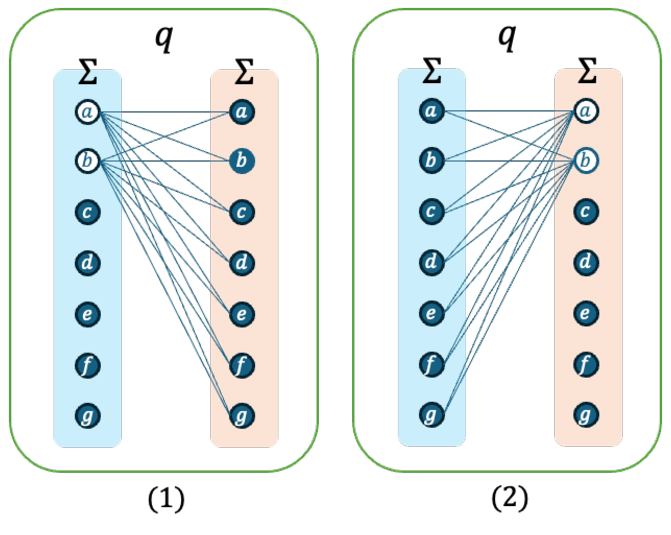
\includegraphics[scale=0.525]{figs/lem4bigraph.pdf}
    \caption{Let $\Sigma=\{a,b,c,d,e,f,g\}$ and $p,q \in \RPat$. We assume that the symbols in $\Sigma$ are mutually distinct.
    These figures express the conditions (i) and (ii) of Lemma~\ref{lem:twovariables} for the cases that (1) $D = \{ ay, by \}$ and (2) $D = \{ ya, yb \}$, respectively.
    In these cases, if $p \{ x := r \} \preceq q$ for all $r \in D$, then $p \{ x := xy \} \preceq q$ holds.}\label{fig:lem4bigraph}
  \end{center}
\end{figure}